%%%%%%%%%%%%%%%%%%%%%%%%%%%%%%%%%%%%%%%%%
% Beamer Presentation
% LaTeX Template
% Version 2.0 (March 8, 2022)
%
% This template originates from:
% https://www.LaTeXTemplates.com
%
% Author:
% Vel (vel@latextemplates.com)
%
% License:
% CC BY-NC-SA 4.0 (https://creativecommons.org/licenses/by-nc-sa/4.0/)
%
%%%%%%%%%%%%%%%%%%%%%%%%%%%%%%%%%%%%%%%%%

%----------------------------------------------------------------------------------------
%	PACKAGES AND OTHER DOCUMENT CONFIGURATIONS
%----------------------------------------------------------------------------------------

\documentclass[
	10pt, % Set the default font size, options include: 8pt, 9pt, 10pt, 11pt, 12pt, 14pt, 17pt, 20pt
	t, % Uncomment to vertically align all slide content to the top of the slide, rather than the default centered
	%aspectratio=169, % Uncomment to set the aspect ratio to a 16:9 ratio which matches the aspect ratio of 1080p and 4K screens and projectors
]{beamer}

\graphicspath{{Images/}{./}} % Specifies where to look for included images (trailing slash required)

\usepackage{booktabs} % Allows the use of \toprule, \midrule and \bottomrule for better rules in tables
\usepackage{graphicx}
\usepackage{caption}
\usepackage{subcaption}
\usepackage{hyperref}
\usepackage[english,brazil]{babel}
\usepackage{fontawesome5}
\usepackage{graphicx}
\usepackage{animate}
\RequirePackage[backend=biber,
style=ieee,
citestyle=authoryear,
]{biblatex}

% Define a custom command for an icon link
\newcommand{\iconLink}[2]{\href{#1}{\faLink \hspace{0.2em} {#2}}}

%----------------------------------------------------------------------------------------
%	SELECT LAYOUT THEME
%----------------------------------------------------------------------------------------
\usetheme{Madrid}

%----------------------------------------------------------------------------------------
%	SELECT COLOR THEME
%----------------------------------------------------------------------------------------

% Beamer comes with a number of color themes that can be applied to any layout theme to change its colors. Uncomment each of these in turn to see how they change the colors of your selected layout theme.

%\usecolortheme{albatross}
%\usecolortheme{beaver}
%\usecolortheme{beetle}
% \usecolortheme{crane}
%\usecolortheme{dolphin}
%\usecolortheme{dove}
%\usecolortheme{fly}
%\usecolortheme{lily}
%\usecolortheme{monarca}
%\usecolortheme{seagull}
%\usecolortheme{seahorse}
%\usecolortheme{spruce}
%\usecolortheme{whale}
%\usecolortheme{wolverine}

%----------------------------------------------------------------------------------------
%	SELECT FONT THEME & FONTS
%----------------------------------------------------------------------------------------
\usefonttheme{default} % Typeset using the default sans serif font

%------------------------------------------------

\usepackage{palatino} % Use the Palatino font for serif text
\usepackage[default]{lato} % Use the Lato font for sans serif text

%----------------------------------------------------------------------------------------
%	SELECT INNER THEME
%----------------------------------------------------------------------------------------
\useinnertheme{rectangles}

%----------------------------------------------------------------------------------------
%	SELECT OUTER THEME
%----------------------------------------------------------------------------------------

% Outer themes change the overall layout of slides, such as: header and footer lines, sidebars and slide titles. Uncomment each theme in turn to see what changes it makes to your presentation.

%\useoutertheme{default}
%\useoutertheme{infolines}
%\useoutertheme{miniframes}
%\useoutertheme{smoothbars}
%\useoutertheme{sidebar}
%\useoutertheme{split}
%\useoutertheme{shadow}
%\useoutertheme{tree}
%\useoutertheme{smoothtree}

%\setbeamertemplate{footline} % Uncomment this line to remove the footer line in all slides
%\setbeamertemplate{footline}[page number] % Uncomment this line to replace the footer line in all slides with a simple slide count

%\setbeamertemplate{navigation symbols}{} % Uncomment this line to remove the navigation symbols from the bottom of all slides

% \bibliography{references} % Specifies the bibliography file to include publications
% \bibliographystyle{apalike} % Specifies the bibliography style
\addbibresource{references.bib}

%----------------------------------------------------------------------------------------
%	PRESENTATION INFORMATION
%----------------------------------------------------------------------------------------

\title[DesWebII]{Desenvolvimento Web II} % The short title in the optional parameter appears at the bottom of every slide, the full title in the main parameter is only on the title page
\subtitle{Aula 04 - Protocolos de Comunicação na Web} % Presentation subtitle, remove this command if a subtitle isn't required
\author[Fabricio Bizotto]{Prof. Fabricio Bizotto} % Presenter name(s), the optional parameter can contain a shortened version to appear on the bottom of every slide, while the main parameter will appear on the title slide
\institute[IFC]{Instituto Federal Catarinense \\ \smallskip \textit{fabricio.bizotto@ifc.edu.br}} % Your institution, the optional parameter can be used for the institution shorthand and will appear on the bottom of every slide after author names, while the required parameter is used on the title slide and can include your email address or additional information on separate lines
\date[\today]{Ciência da Computação \\ \today} % Presentation date or conference/meeting name, the optional parameter can contain a shortened version to appear on the bottom of every slide, while the required parameter value is output to the title slide

%----------------------------------------------------------------------------------------
\begin{document}

%----------------------------------------------------------------------------------------
%	TITLE SLIDE
%----------------------------------------------------------------------------------------

\begin{frame}
	\titlepage % Output the title slide, automatically created using the text entered in the PRESENTATION INFORMATION block above
\end{frame}

%----------------------------------------------------------------------------------------
%	TABLE OF CONTENTS SLIDE
%----------------------------------------------------------------------------------------

\begin{frame}
	\frametitle{Roteiro} % Slide title, remove this command for no title
	
	\tableofcontents % Output the table of contents (all sections on one slide)
	%\tableofcontents[pausesections] % Output the table of contents (break sections up across separate slides)
\end{frame}

%----------------------------------------------------------------------------------------
%	PRESENTATION BODY SLIDES
%----------------------------------------------------------------------------------------

\section{Protocolos de Comunicação} % Sections are added in order to organize your presentation into discrete blocks, all sections and subsections are automatically output to the table of contents as an overview of the talk but NOT output in the presentation as separate slides

%------------------------------------------------

\subsection{Conceito}

\begin{frame}
	\frametitle{Conceito}

	Protocolo de comunicação é um conjunto de regras que definem como a comunicação entre dois ou mais dispositivos deve ocorrer. Existem diversos protocolos de comunicação, cada um com suas características e finalidades específicas. Alguns exemplos de protocolos de comunicação são:

	\begin{itemize}
		\item \textbf{HTTP} - \textit{Hypertext Transfer Protocol}
		\item \textbf{HTTPS} - \textit{Hypertext Transfer Protocol Secure}
		\item \textbf{FTP} - \textit{File Transfer Protocol}
		\item \textbf{SMTP} - \textit{Simple Mail Transfer Protocol}
		\item \textbf{SSH} - \textit{Secure Shell}
		\item \textbf{Websocket} - \textit{Websocket Protocol}
	\end{itemize}

\end{frame}

%------------------------------------------------

\subsection{HTTP}

\begin{frame}
	\begin{center}
		
		\bigskip\bigskip\bigskip\bigskip % Vertical whitespace
		{\Large Protocolos de Comunicação}
		
		\bigskip\bigskip % Vertical whitespace
		{\Huge HTTP}
		
		\smallskip
		{\small \textit{Hypertext Transfer Protocol}}
	\end{center}

\end{frame}

\begin{frame}
	\frametitle{HTTP}
	
	\begin{itemize}
		\item \alert{Protocolo} de comunicação utilizado para transferência de dados na \textbf{World Wide Web} (WWW).
		\item Utiliza o protocolo \textbf{TCP}, normalmente na porta \textbf{80}.
		\item É um protocolo \textbf{stateless}, ou seja, não mantém estado entre requisições.
		\item É um protocolo \textbf{client-server}, ou seja, o cliente envia uma requisição e o servidor responde.
		\item A \textbf{URL} é utilizada para identificar o recurso que será acessado pelo cliente (browser, por exemplo).
		\item \alert{Local Storage e Cookies} são utilizados para manter estado entre requisições e melhorar a experiência do usuário.
	\end{itemize}

\end{frame}

\subsubsection{Métodos HTTP}

\begin{frame}
	\frametitle{HTTP - Métodos}

	\begin{figure}
		\centering
		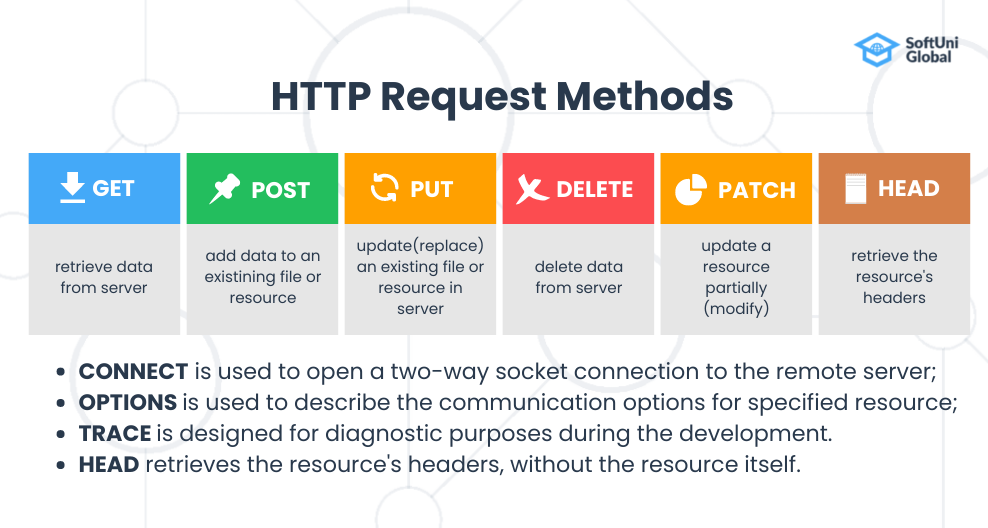
\includegraphics[width=0.9\linewidth]{methods.png}
		\caption{Métodos HTTP \footnote{\iconLink{https://pbs.twimg.com/media/F3Aak4jXoAAl4-y?format=jpg&name=large}{Twitter Post: Top 9 HTTP Request Methods}}.}
		\label{fig:httpmethods}
	\end{figure}

\end{frame}

\subsubsection{Códigos de Status}

\begin{frame}
	\frametitle{HTTP - Códigos de Status}

	\begin{figure}
		\centering
		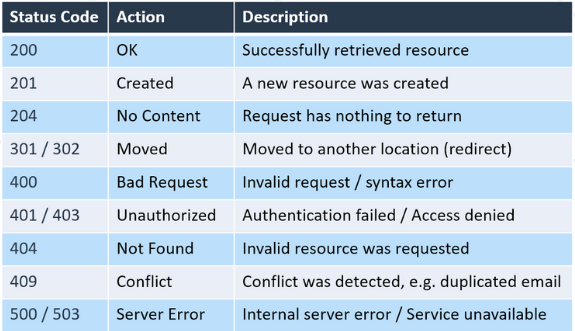
\includegraphics[width=0.9\linewidth]{status_code.png}
		\caption{Códigos de status HTTP.}
		\label{fig:status}
	\end{figure}

\end{frame}

\subsubsection{Requisição e Resposta}

\begin{frame}
	\frametitle{HTTP - Requisição e Resposta}

	\begin{figure}
		\centering
		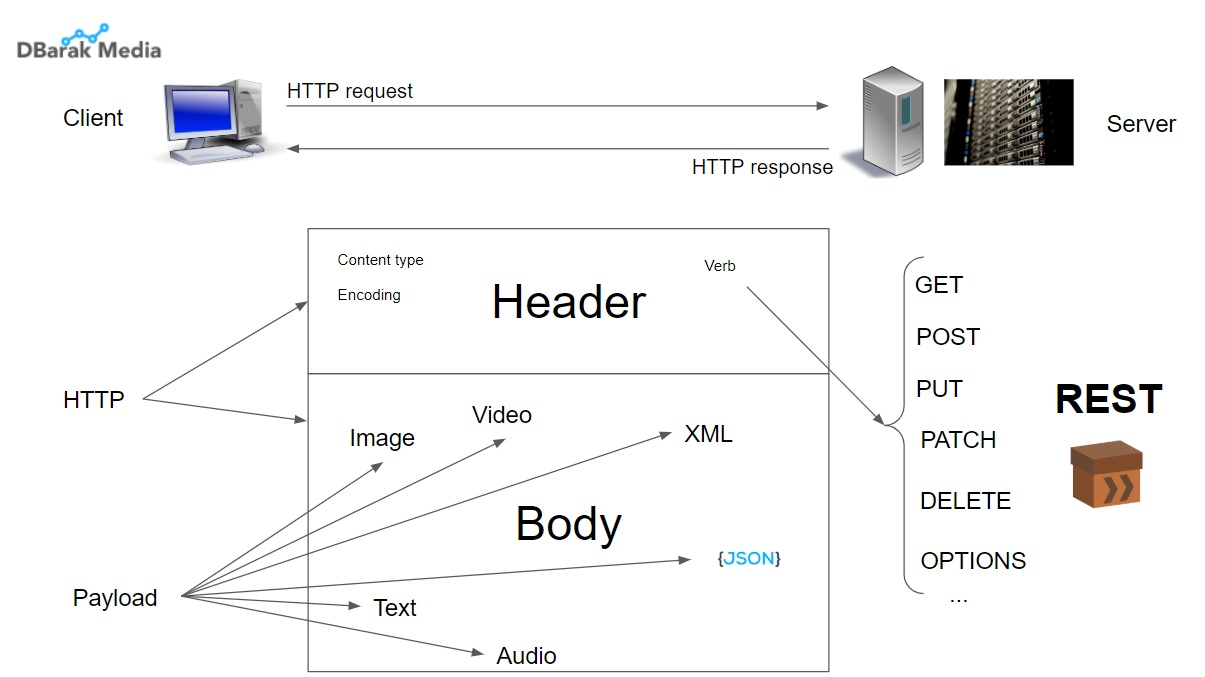
\includegraphics[width=0.9\linewidth]{http_explained.jpg}
		\caption{Ilustração do funcionamento do protocolo HTTP.}
		\label{fig:http}
	\end{figure}

\end{frame}

\begin{frame}
	\frametitle{HTTP - Requisição e Resposta}

	\begin{figure}
		\centering
		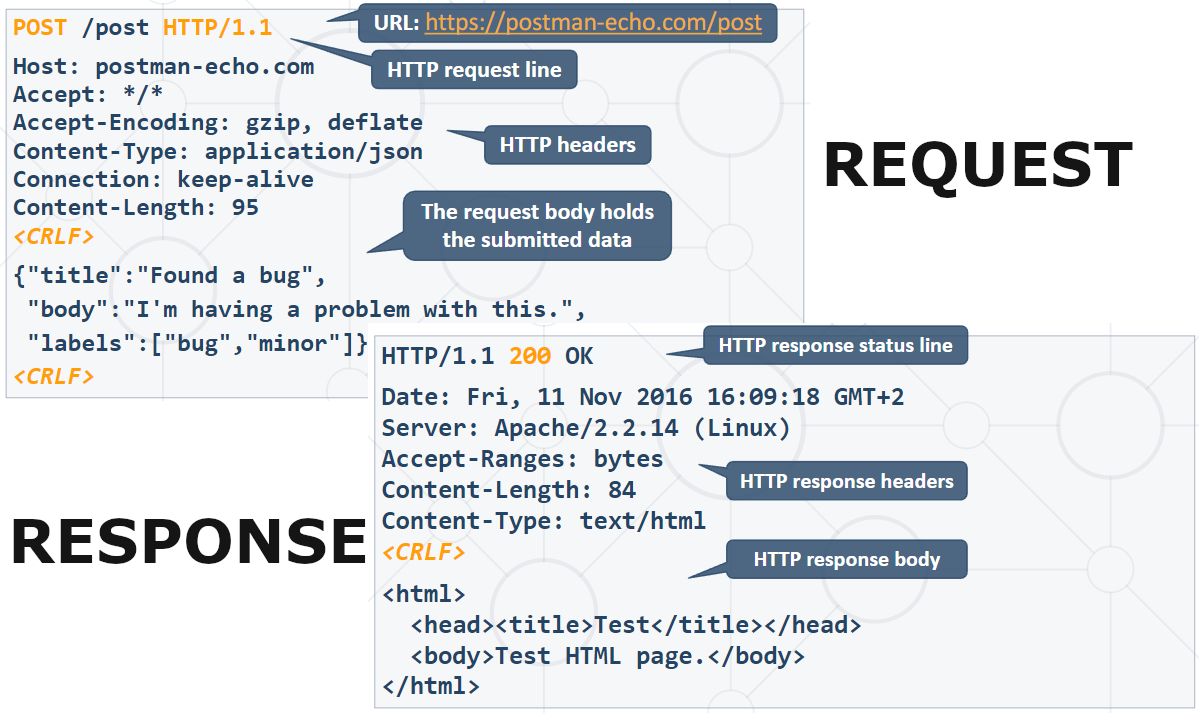
\includegraphics[width=0.9\linewidth]{req_res.png}
		\caption{Requisição e resposta HTTP.}
		\label{fig:http_req_res}
	\end{figure}

\end{frame}

\subsection{HTTPS}
\setcounter{footnote}{0}

\begin{frame}
	\frametitle{HTTPS}

	\begin{itemize}
		\item \textbf{HTTPS} - \textit{Hypertext Transfer Protocol \alert{Secure}}.
		\item Os dados são criptografados antes de serem enviados. Evita que os dados sejam modificados durante a transmissão.
		\item Utiliza o protocolo \textbf{SSL} - \textit{Secure Sockets Layer} ou \textbf{TLS} - \textit{Transport Layer Security}.
		\item O certificado SSL/TLS (criptografia assimétrica) é emitido por uma \textbf{AC} - \textit{Autoridade Certificadora} e instalado no servidor \footnote{\iconLink{https://letsencrypt.org/}{Let's Encrypt}}.
	\end{itemize}
	
	\begin{block}{O que HTTPS não faz?}
		\begin{itemize}
			\item Não garante que o servidor é confiável.
			\item Não garante que o servidor não foi invadido.
			\item Não garante que o servidor não está enviando dados para terceiros.
			\item Não oculta o endereço do site que está sendo acessado.
			\item Não esconde sua identidade e localização.
			\item Não evita que o usuário pegue vírus. Não é um filtro de conteúdo.
		\end{itemize}
		
	\end{block}
	
\end{frame}

\begin{frame}
	\frametitle{HTTPS}

	\begin{figure}
		\centering
		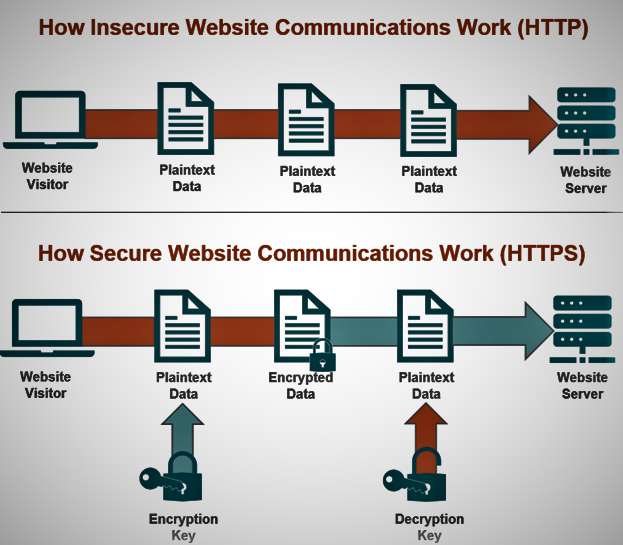
\includegraphics[width=0.65\linewidth]{http_https.png}
		\caption{Comparação entre o funcionamento do protocolo HTTP e HTTPS.}
		\label{fig:https}
	\end{figure}

\end{frame}

\begin{frame}
	\frametitle{HTTPS - Consultando o Certificado}

	\begin{figure}
		\centering
		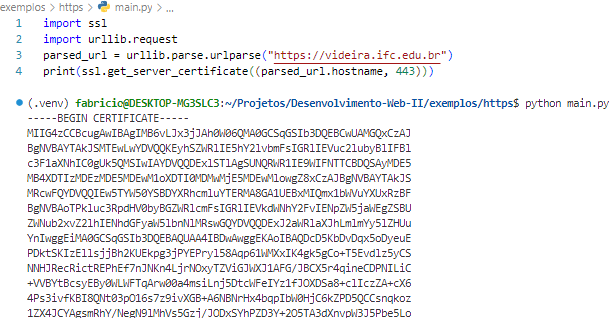
\includegraphics[width=0.9\linewidth]{ssl_consulta.png}
		\caption{Consultando o certificado SSL/TLS.}
		\label{fig:https_ssl}
	\end{figure}

\end{frame}


\begin{frame}
	\frametitle{HTTPS - Criando e consumindo meu próprio certificado}

	\begin{figure}
		\centering
		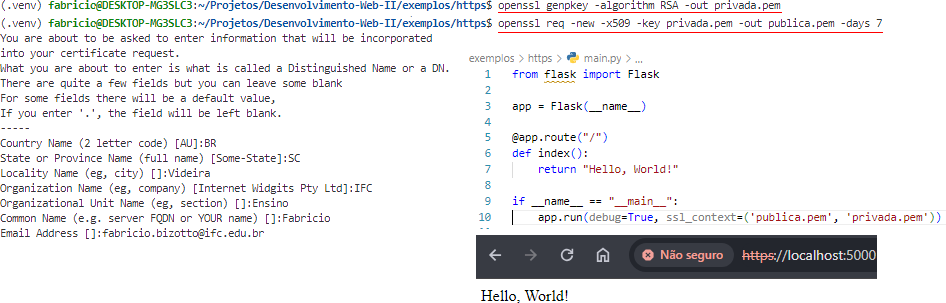
\includegraphics[width=0.9\linewidth]{ssl_python_example.png}
		\caption{Criando e consumindo meu próprio certificado.}
		\label{fig:https_ssl_example}
	\end{figure}

\end{frame}

\subsection{Websocket}

\begin{frame}
	\begin{center}
		
		\bigskip\bigskip\bigskip\bigskip % Vertical whitespace
		{\Large Protocolos de Comunicação}
		
		\bigskip\bigskip % Vertical whitespace
		{\Huge Web Socket}
		
		\smallskip
		{\small \textit{Web Socket Protocol}}
	\end{center}

\end{frame}

\begin{frame}
	\frametitle{Antes de Websocket}

	\begin{figure}
		\centering
		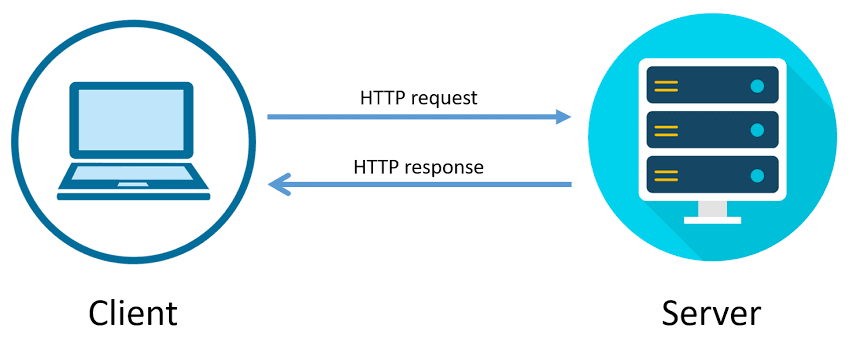
\includegraphics[width=0.5\linewidth]{http_padrao.png}
		\caption{Fluxo normal de requisição e resposta HTTP.}
		\label{fig:http_padrao}
	\end{figure}

	\begin{itemize}
		\item \textbf{Pooling} - O cliente faz requisições ao servidor em intervalos regulares. O servidor responde, mesmo que não tenha novos dados.
		\item \textbf{Long polling} - O cliente faz uma requisição e o servidor mantém a conexão aberta até que tenha novos dados. O servidor responde quando tiver novos dados ou quando o tempo limite for atingido.
		\item \alert{Essas abordagens são ineficientes e consomem muitos recursos. Cada requisição/resposta gera um \textit{overhead} de comunicação.}
	\end{itemize}

\end{frame}

\begin{frame}
	\frametitle{HTTP - Estratégia de Pooling}

	\begin{figure}
		\centering
		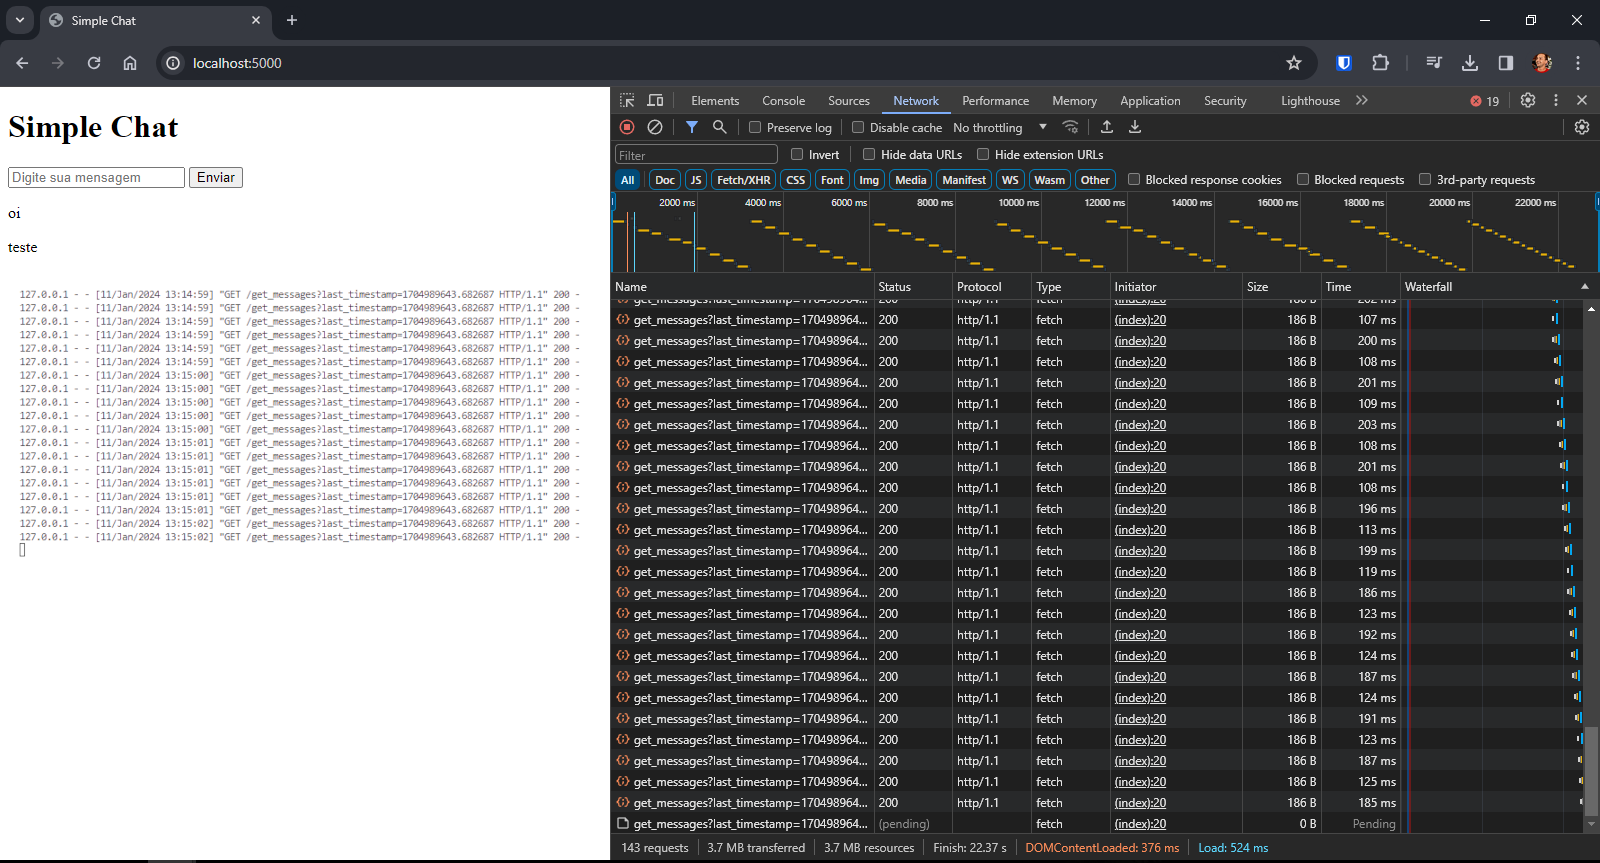
\includegraphics[width=0.9\linewidth]{pooling.png}
		\caption{HTTP - Pooling.}
		\label{fig:http_pooling}
	\end{figure}
	
\end{frame}

\begin{frame}
	\frametitle{Web Socket}

	\begin{itemize}
		\item É um protocolo de comunicação \textbf{full-duplex}, ou seja, permite que o cliente e o servidor enviem dados simultaneamente.
		\item Utiliza o protocolo \textbf{TCP}, normalmente na porta \textbf{443}.
		\item É um protocolo \textbf{stateful}, ou seja, mantém estado entre requisições.
		\item A comunicação é iniciada com um \textbf{handshake} HTTP para garantir ambas as partes concordam em estabelecer uma conexão bidirecional persistente.
		\item Muito usado em aplicações que precisam de comunicação em tempo real, tais como: 
		\begin{itemize}
			\item \textbf{Chat}
			\item \textbf{Jogos}
			\item \textbf{Streaming}
			\item \textbf{Gráfico de ações em tempo real}
			\item \textbf{etc}
		\end{itemize}
	\end{itemize}

	\begin{alertblock}{Onde não usar?}
		Não é recomendado usar em situações onde a comunicação é pontual ou para buscar dados antigos. Nesses casos, o HTTP é mais adequado.
	\end{alertblock}


\end{frame}

\begin{frame}
	\frametitle{Web Socket - Diagrama de funcionamento}

	\begin{figure}
		\centering
		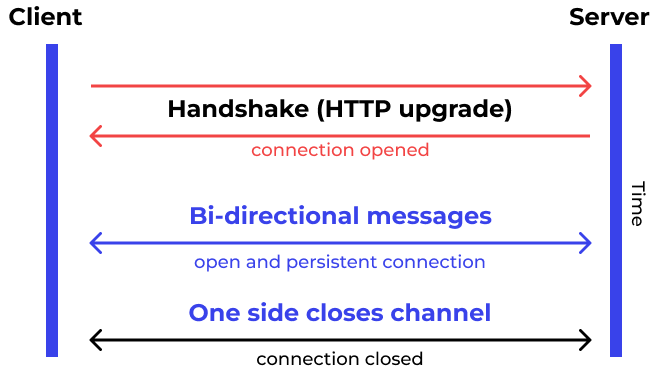
\includegraphics[width=0.9\linewidth]{websocket.png}
		\caption{Diagrama de funcionamento do protocolo Websocket.}
		\label{fig:websocket}
	\end{figure}

\end{frame}

\begin{frame}
	\frametitle{Web Socket - Exemplo de uso}

	\begin{figure}
		\centering
		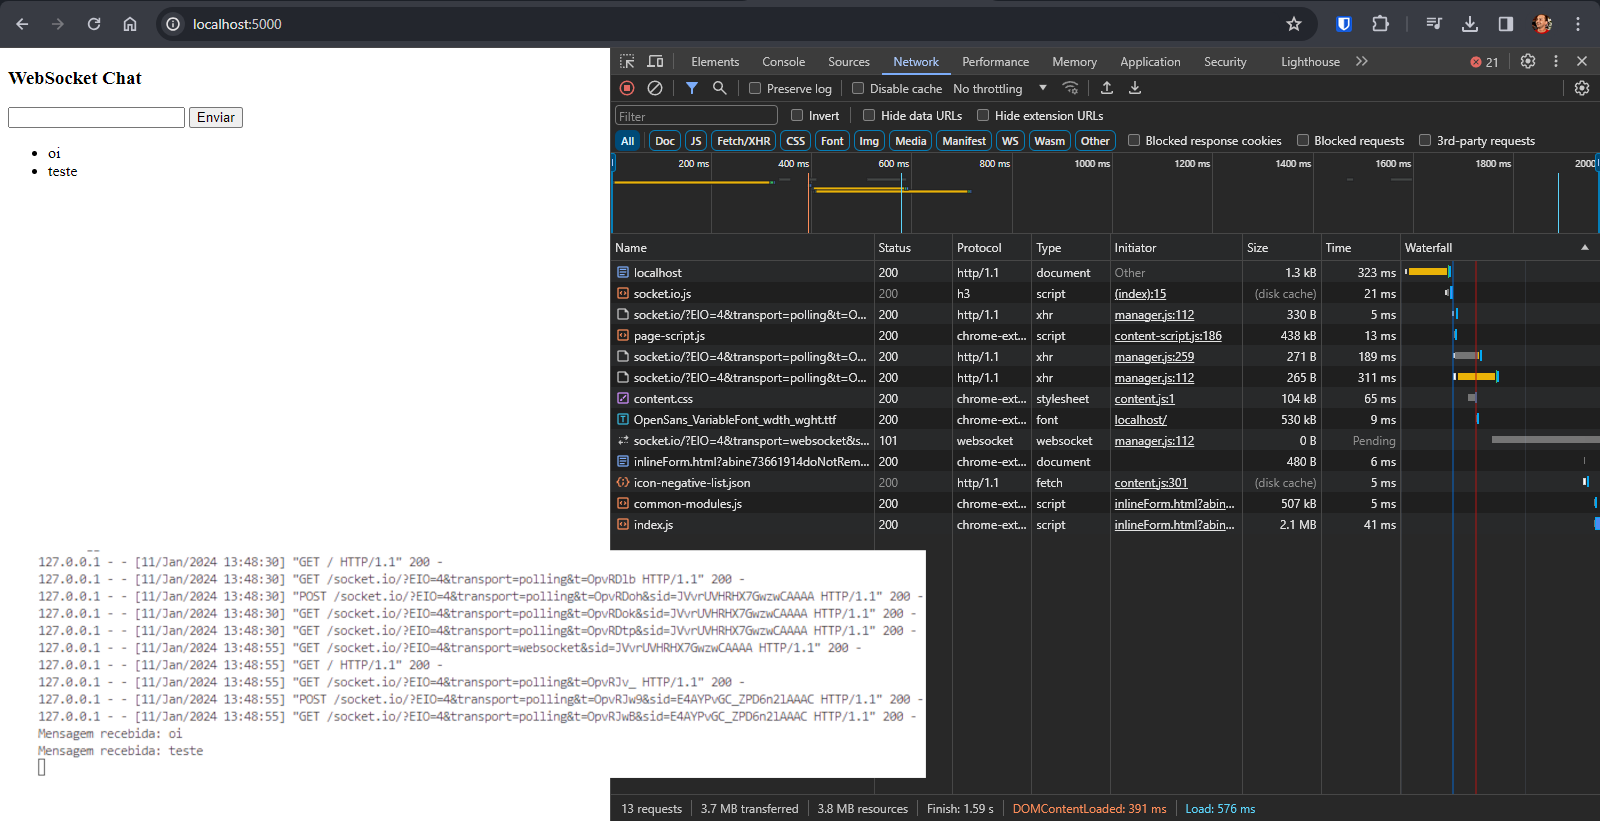
\includegraphics[width=0.9\linewidth]{websocket_example.png}
		\caption{Exemplo de uso do protocolo Websocket.}
		\label{fig:websocket_example}
	\end{figure}

\end{frame}

\begin{frame}
	\frametitle{Comparação entre HTTP e Websocket}

	\begin{figure}
		\centering
		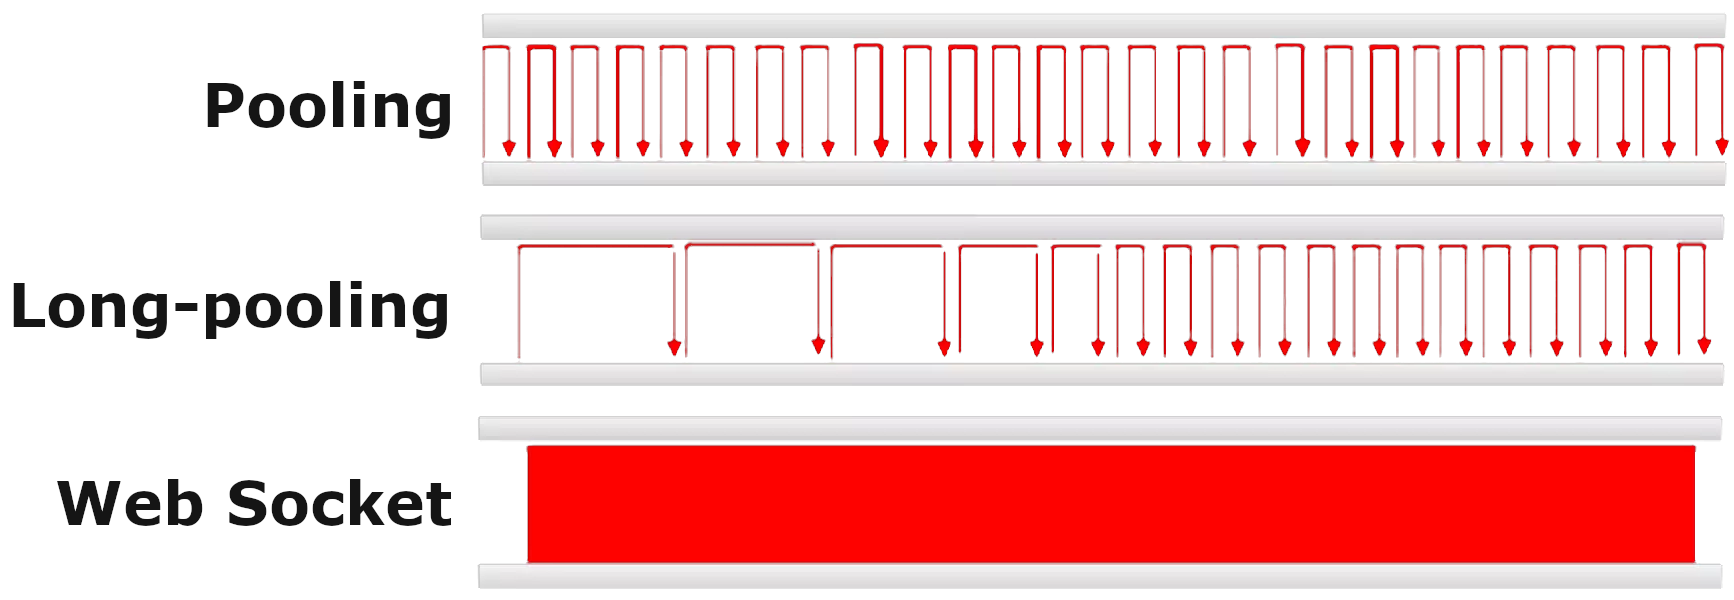
\includegraphics[width=0.8\linewidth]{po_lp_ws.png}
		\caption{Comparação entre Pooling, Long Polling e Websocket.}
		\label{fig:websocket_example2}
	\end{figure}

	\begin{figure}
		\centering
		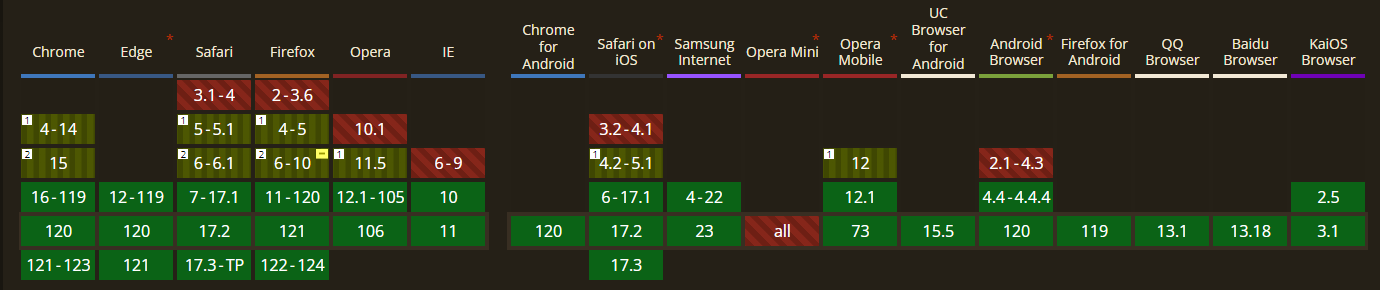
\includegraphics[width=0.8\linewidth]{ws_support.png}
		\caption{Can I use: - Web Socket Browser Support.}
		\label{fig:websocket_support}
	\end{figure}

\end{frame}

\section{Material Complementar}

\begin{frame}
	\frametitle{Material Complementar}

	\href{https://codepen.io/matt-west/pen/nYvVBV}{\faLink \hspace{0.2em} Web Socket - Demo}\\
	\href{https://www.hipsters.tech/http2-magia-com-o-novo-protocolo}{\faPodcast \hspace{0.2em} HTTP2: magia com o novo protocolo – Hipsters (2016)}\\
	\href{https://www.hipsters.tech/web3-vale-o-hype-hipsters-ponto-tech-380}{\faPodcast \hspace{0.2em} Web3 vale o hype? – Hipsters (2023)}\\
	\href{https://www.casadocodigo.com.br/products/livro-desconstruindo-web}{\faBook \hspace{0.2em} Desconstruindo a Web: As tecnologias por trás de uma requisição}\\

\end{frame}

% \section{Tarefa}

% \begin{frame}
% 	\frametitle{Tarefa}

% 	\begin{enumerate}
% 		\item Explique as principais diferenças entre HTTP e HTTPS em termos de segurança.
% 		\item Descreva como funciona o processo de criptografia no HTTPS e por que é importante para a segurança da comunicação web.
% 		\item Explique o processo de handshake SSL/TLS no estabelecimento de uma conexão HTTPS.
% 		\item Defina o conceito de Web Sockets e explique como ele se diferencia do modelo de solicitação-resposta do HTTP. Cite exemplos de aplicações que podem se beneficiar do uso de Web Sockets.
% 		\item Destaque as melhorias específicas introduzidas pelo HTTP/2 em relação à versão anterior.
% 	\end{enumerate}

% 	\begin{alertblock}{Entrega}
% 		\begin{itemize}
% 			\item Formato: Escrito a mão.
% 			\item Prazo: no início da próxima aula.
% 		\end{itemize}
% 	\end{alertblock}

% \end{frame}

\section{Experimentos}

\begin{frame}
	\frametitle{Experimentos}


	\begin{exampleblock}{Lista de Experimentos}
		% pular linha
		Escolha um dos experimentos abaixo para realizar:\\
		\href{https://gist.github.com/fabricioifc/e620122192af1abca4fe22e6fdd9bce3}{\faLink \hspace{0.2em} Lista de Experimentos}
	\end{exampleblock}
	


	% \begin{alertblock}{Entrega}
	% 	\begin{itemize}
	% 		\item Formato: Link do código-fonte publicado no GitHub (README.md: adicione instruções de como executar a aplicação).
	% 		\item Plataforma: SIGAA.
	% 		\item Prazo: no início da próxima aula.
	% 	\end{itemize}
	% \end{alertblock}

\end{frame}

	

%----------------------------------------------------------------------------------------
%	CLOSING SLIDE
%----------------------------------------------------------------------------------------

% \begin{frame}[plain] % The optional argument 'plain' hides the headline and footline
% 	\begin{center}
% 		\bigskip\bigskip % Vertical whitespace
		
% 		{\Huge Perguntas? Comentários?}
		
% 		\bigskip\bigskip % Vertical whitespace
		
% 		{\LARGE Aula 04 - Protocolos de Comunicação na Web}
% 	\end{center}
% \end{frame}

%----------------------------------------------------------------------------------------

\end{document} 